%
% kettenloesung.tex -- template for standalon tikz images
%
% (c) 2020 Prof Dr Andreas Müller, Hochschule Rapperswil
%
\documentclass[tikz]{standalone}
\usepackage{amsmath}
\usepackage{times}
\usepackage{txfonts}
\usepackage{pgfplots}
\usepackage{csvsimple}
\usetikzlibrary{arrows,intersections,math}
\def\skala{3.2}
\begin{document}
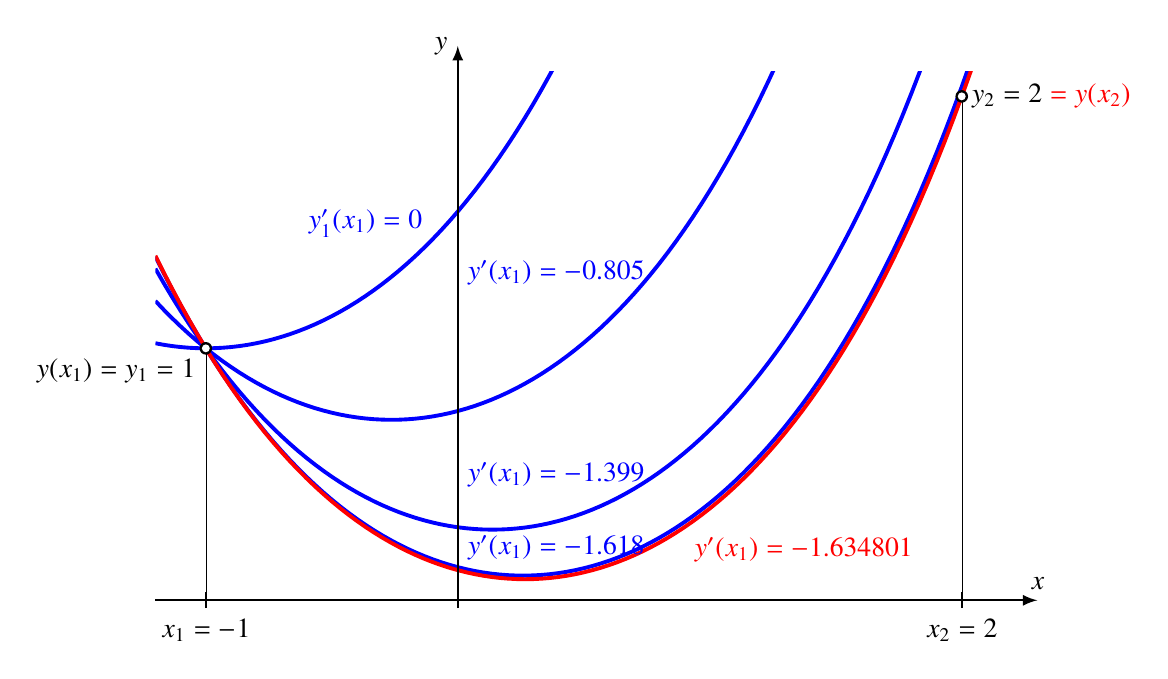
\begin{tikzpicture}[>=latex,thick,scale=\skala]

\def\kurvenparameter#1{
	\xdef\m{#1}
	\pgfmathparse{ln(\m+sqrt(1+\m*\m))}
	\xdef\am{\pgfmathresult}
}

\def\kurve#1#2{
	\kurvenparameter{#1}
	\draw[color=#2,line width=1.4pt]
		plot[domain=-1.2:2.1,samples=100]
			({\x},{0.5*(exp(\x+1+\am)+exp(-\x-1-\am))+1-sqrt(1+\m*\m)});
}

\begin{scope}
\clip (-1.2,0) rectangle (2.1,2.1);
\kurve{0}{blue}
\kurve{-0.805}{blue}
\kurve{-1.399}{blue}
\kurve{-1.618}{blue}
\kurve{-1.634801}{red}
\end{scope}

\node[color=blue] at (-0.1,1.4) [above left] {$y_1'(x_1)=0$};
\node[color=blue] at (0,1.3) [right] {$y'(x_1)=-0.805$};
\node[color=blue] at (0,0.5) [right] {$y'(x_1)=-1.399$};
\node[color=blue] at (0,0.21) [right] {$y'(x_1)=-1.618$};
\node[color=red] at (0.9,0.2) [right] {$y'(x_1)=-1.634801$};

% Koordinatenachsen
\draw[->] (-1.2,0)--(2.3,0) coordinate[label={$x$}];
\draw[->] (0,{-0.1/\skala})--(0,2.2) coordinate[label={left:$y$}];

% ticks an den Endpunkten
\draw[line width=0.1pt] (-1,0)--(-1,1);
\draw (-1,{-0.1/\skala})--(-1,{0.1/\skala});
\node at (-1,{-0.1/\skala}) [below] {$x_1=-1$};

\draw[line width=0.1pt] (2,0)--(2,2);
\draw (2,{-0.1/\skala})--(2,{0.1/\skala});
\node at (2,{-0.1/\skala}) [below] {$x_2=2$};

\node at (-1,1) [below left] {$y(x_1)=y_1=1$};
\node at (2,2) [right] {$y_2=2{\color{red}\mathstrut =y(x_2)}$};

\fill (-1,1) circle[radius={0.08/\skala}];
\fill[color=white] (-1,1) circle[radius={0.05/\skala}];

\fill (2,2) circle[radius={0.08/\skala}];
\fill[color=white] (2,2) circle[radius={0.05/\skala}];

\end{tikzpicture}
\end{document}

